\documentclass{exam}

\usepackage{units} 
\usepackage{graphicx}
\usepackage[fleqn]{amsmath}
\usepackage{cancel}
\usepackage{float}
\usepackage{mdwlist}
\usepackage{booktabs}
\usepackage{cancel}
\usepackage{polynom}
\usepackage{caption}
\usepackage{fullpage}
\usepackage{xfrac}
\usepackage{enumerate}

\newcommand{\degree}{\ensuremath{^\circ}} 
\everymath{\displaystyle}

% \printanswers

% \begin{figure}[H]
%   \centering
%   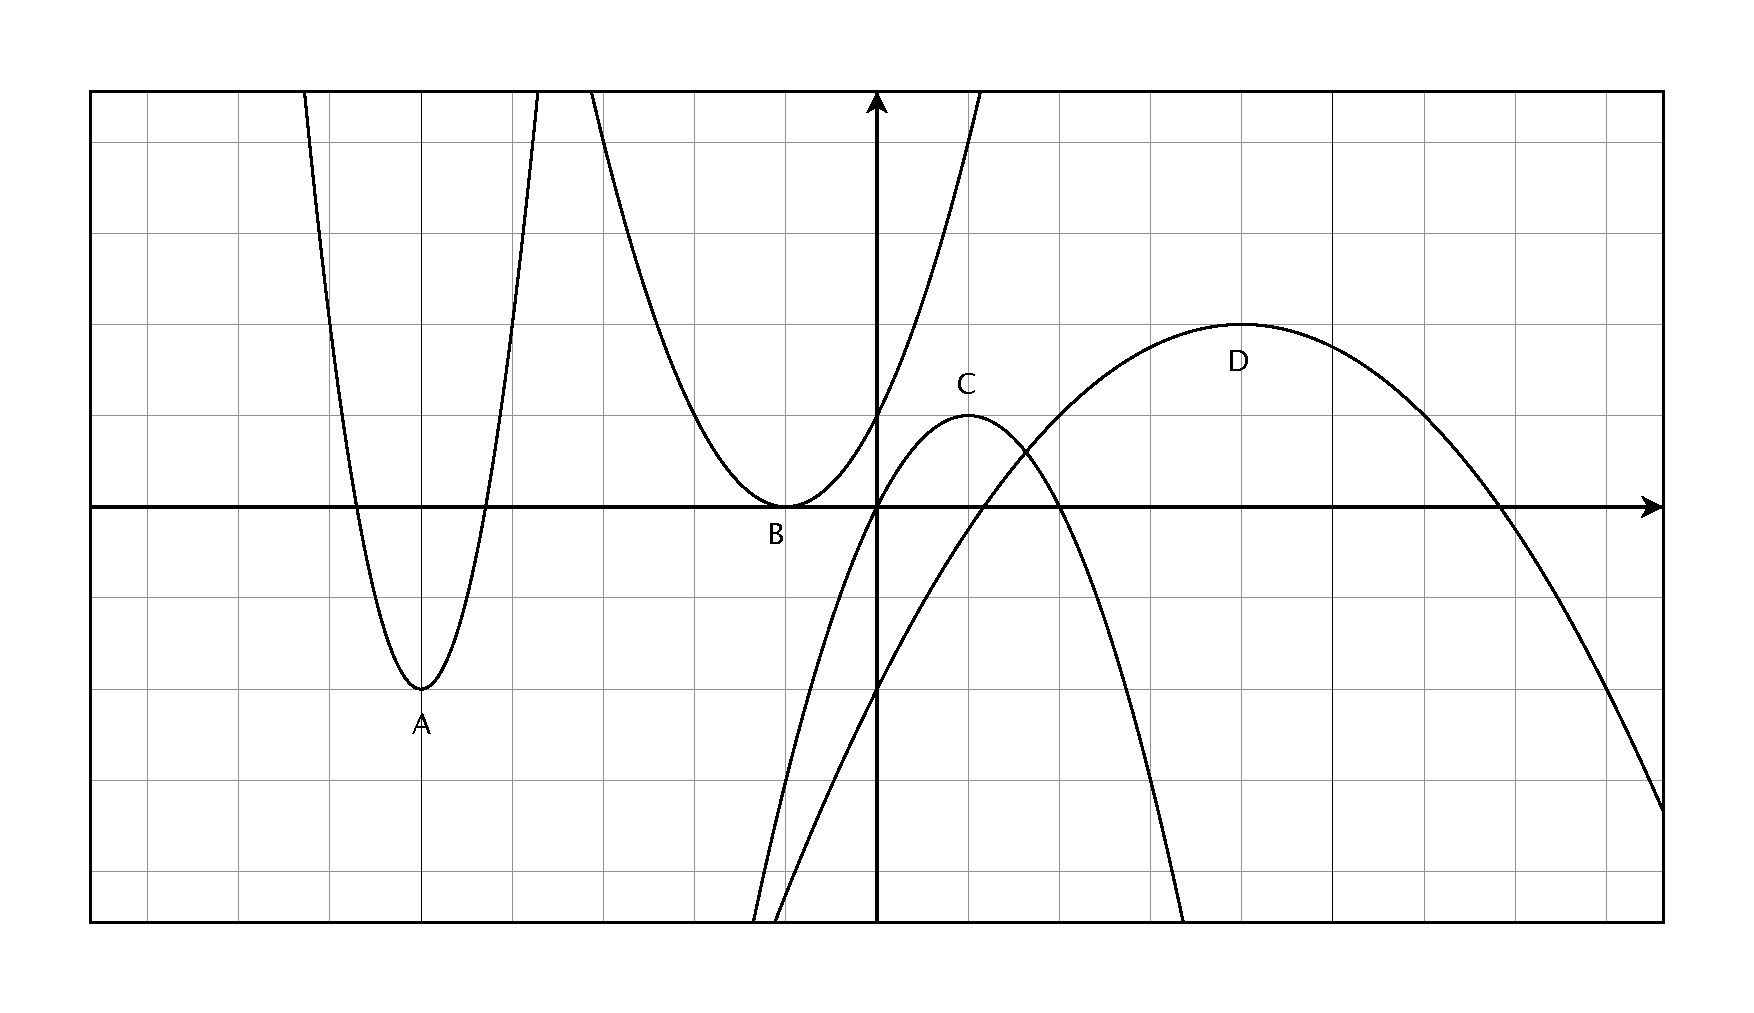
\includegraphics[scale=.3]{problem_7.eps}
%   \caption*{Problem 7}
% \end{figure}

% \begin{tabular}{cc}
% \toprule
% period & amplitude \\
% \midrule
%   $\pi$ & $2$ \\
% \bottomrule
% \end{tabular}

\title{Math 141 \\ Section 3.5 Examples}
\date{May 1, 2013}

\begin{document}

\maketitle

\begin{questions}

  \uplevel{For questions \ref{factor:first} to \ref{factor:last}, factor each polynomial completely}

  \question $f(x) = x^3+2 x^2+x+2$ 
  \label{factor:first}

    \begin{solution}
        $x = \left\{ \pm i, -2 \right\}$ 
    \end{solution}

  \question $f(x) = x^3-3 x^2+2 x+6$ 
    \begin{solution}
      $x = {-1, 2 \pm i \sqrt{2}}$ 
    \end{solution}

  \question $f(x) = x^4-4 x^3+8 x^2-16 x+16$
    \begin{solution}
      $x = {2, \pm 2i}$
    \end{solution}

  \question $f(x) = x^4-x^3-7 x^2+8 x+4$
    \begin{solution}
      $x = \left\{ 2, \frac{1}{2} \left(-3 \pm \sqrt{5}\right) \right\}$
    \end{solution}

  \question $f(x) = x^5 - 9x$ 
  \label{factor:last}
    \begin{solution}
      $x = \left\{ 0, \pm \sqrt{3}, \pm i \sqrt{3} \right\}$ 
    \end{solution}

  \question Find a polynomial with degree 3 and zeros 2 and $i$
    \begin{solution}
      $f(x) = x^3-2 x^2+x-2$
    \end{solution}

  \ifprintanswers
    \pagebreak
  \fi

  \question Find a polynomial with degree 4 and zeros 1 and $2 - i$
    \begin{solution}
      $f(x) = x^4-6 x^3+14 x^2-14 x+5$
    \end{solution}
\end{questions}

\end{document}
